%Dokumentinformationen
\newcommand{\titleinfo}{Complexe Zahlen, Fourierreihen - Formelsammlung}
\newcommand{\authorinfo}{F. Braun, L. Schmid, U. Giger, R. Koller, E. Ammann, S.
Arnold}
\newcommand{\versioninfo}{$Revision: 878 $ - powered by \LaTeX}

% standard header
%Schriftgr�sse, Layout, Papierformat, Art des Dokumentes
\documentclass[10pt,twoside,a4paper,fleqn]{article}
%Einstellungen der Seitenr�nder
\usepackage[left=1cm,right=1cm,top=1cm,bottom=1cm,includeheadfoot]{geometry}
% Sprache, Zeichensatz, packages
\usepackage[utf8]{inputenc}
\usepackage[ngerman]{babel,varioref}
\usepackage{amssymb,amsmath,fancybox,graphicx,color,lastpage,wrapfig,fancyhdr,hyperref,verbatim}

%pdf info
\hypersetup{pdfauthor={\authorinfo},pdftitle={\titleinfo},colorlinks=false}
%linkbordercolor=white
\author{\authorinfo}
\title{\titleinfo}

%Kopf- und Fusszeile
\pagestyle{fancy}
\fancyhf{}
%Linien oben und unten
\renewcommand{\headrulewidth}{0.5pt} 
\renewcommand{\footrulewidth}{0.5pt}

\fancyhead[L]{\titleinfo{ }\tiny{(\versioninfo)}}
%Kopfzeile rechts bzw. aussen
\fancyhead[R]{Seite \thepage { }von \pageref{LastPage}}
%Fusszeile links bzw. innen
\fancyfoot[L]{\footnotesize{\authorinfo}}
%Fusszeile rechts bzw. ausen
\fancyfoot[R]{\footnotesize{\today}} % ./header.tex nicht editieren (Projekt LaTeX-Header benutzen)

%%%%%%%%%%%%%%%%%%%%%%%%%%%%%%%%%%%%%%%%%%%%%%%%%%%%%%%%%%%%%%%%%%%%%%%%%%%%%%%%%%%%%%%%%%%%%%%%
% Neue Befehle und Definitionen                
%%%%%%%%%%%%%%%%%%%%%%%%%%%%%%%%%%%%%%%%%%%%%%%%%%%%%%%%%%%%%%%%%%%%%%%%%%%%%%%%%%%%%%%%%%%%%%%%
\definecolor{black}{rgb}{0,0,0} 
\definecolor{red}{rgb}{1,0,0}
\definecolor{white}{rgb}{1,1,1}
\definecolor{grey}{rgb}{0.8,0.8,0.8}
\newcommand{\verweis}[2]{\small{(siehe auch \ref{#1}, #2 (S. \pageref{#1}))}}

% Titel
\newcommand{\skriptsection}[2]{\section{#1 {\tiny Skript S. #2}}}
\newcommand{\skriptsubsection}[2]{\subsection{#1 {\tiny Skript S. #2}}}
\newcommand{\skriptsubsubsection}[2]{\subsubsection{#1 {\tiny Skript S. #2}}}

% Mathematische Operatoren
\DeclareMathOperator{\cjs}{cjs}
\DeclareMathOperator{\Ln}{Ln}


\begin{document}
\setlength{\parindent}{0pt}

\skriptsection{Complexe Zahlen}{1}
\skriptsubsection{Grundlagen}{1ff}
\begin{minipage}[t]{9.4cm}
	\textbf{Cartesische Form}\\
	Normalform: $z = z_1 +j z_2$\\
	$z_1 = \text{Re}(z), \quad z_2 = \text{Im}(z)$\\
	Umrechnung in Polar:\\
	$r = |z| = \sqrt{z_1^2 + z_2^2}, \quad 
	\varphi = 	\begin{cases} 
                	\arctan(\frac{z_2}{z_1}) &z_1 \geq 0\\
                	\arctan(\frac{z_2}{z_1}) + \pi &z_1 < 0
    			\end{cases}$
\end{minipage}
\begin{minipage}[t]{9.4cm}
	\textbf{Polarsystem}\\
	Normalform: 
	$z = r \cjs(\varphi) = r(\cos{\varphi} + j\sin{\varphi}) = r e^{j \varphi}$\\
	$\varphi = \arg(z)$

	Umrechnung in Cartesisch:\\
	$z_1 = |z| \cos{\varphi}, \quad z_2 = |z| \sin{\varphi}$
\end{minipage}
\begin{center}
{\textbf{Imaginäre Einheit} $\qquad j^2 = -1 \qquad e^{j\pi} = -1 \qquad
\frac{1}{j} = -j$}
\end{center}

\skriptsubsection{Rechenregeln}{10ff}
\begin{tabular}{ll}
$+, -$
&Selbige Regeln wie für $\mathbb{R}$\\

Mulitplikation
&$a \cdot b = 
|a| |b| \cjs(\alpha + \beta) = 
|a| |b| e^{j(\alpha + \beta)}$\\

Division
&$\left|\frac{a}{b}\right| = 
\frac{\left|a\right|}{\left|b\right|} \cjs(\alpha - \beta) =
\frac{\left|a\right|}{\left|b\right|} e^{j(\alpha - \beta)}$ (cartesisch: Mit
conj. complex des Nenners erweitern) \\

Conjugiert complex
&$\overline{z} = \overline{z_1 + jz_2} = z_1 - jz_2; \qquad \qquad z \cdot \overline{z} = |z|^2$\\

Wurzeln
&$\sqrt[n]{a} = \sqrt[n]{|a|} \cjs(\frac{arg(a)}{n}+k\frac{2\pi}{n}) = 
\sqrt[n]{|a|} e^{j(\frac{\alpha}{n} + k \frac{2\pi}{n})} \quad (k = 0, 1,
\ldots, n-1 \Rightarrow \text{n Lösungen in } \mathbb{C} !)$ \\

Potenzen
&$a^n = |a|^n \cjs(n\alpha) = 
|a|^n e^{jn\alpha}$\\

$e^z$ &$e^{z_1+jz_2} = e^{z_1} \cjs(z_2) = e^{z_1} (\cos{z_2} + j\sin{z_2})$\\

Moivre'sche Formel
&$\text{cjs}^n(\varphi) =
(\cos{\varphi} + j\sin{\varphi})^n = 
\cos(n\varphi) +j\sin(n\varphi) \quad (n \in \mathbb{N})$\\

Logarithmus
&$Ln(z) = \ln{|z|} + j (\arg(z) + 2k \pi)$
\end{tabular}

\begin{minipage}[t]{11.4cm}
	\textbf{Bemerkungen}\\
	\begin{itemize}
	  \item $p_n(z) \; (n \geq 1, z \in \mathbb{C})$ hat $n$ Lösungen und Nullstellen (in
	$\mathbb{C}$)  
	  \item Allgemeine Potenzen $a^b,\;a,b \in \mathbb{C}$ können mit $e^{b \cdot 
	  Ln(a)}$ und den bekannten für $\mathbb{R}$ gültigen Potenzregeln gelöst
	  werden.
	  \item Re$\left (\frac{a}{b} \right) = 0$: Die beiden compl. Zahlen $a, b$
	  stehen senkrecht zueinander.
	\end{itemize}
\end{minipage}
\begin{minipage}[t]{7.4cm}
	\textbf{Einheitswurzeln}\\
	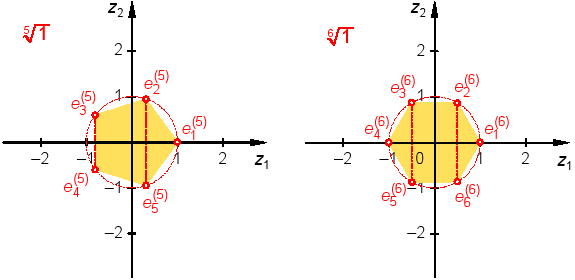
\includegraphics[width=7cm]{./bilder/einheitswurzel.png}
\end{minipage}
\subsection{12. Einheitswurzeln ($k 30 \symbol{23}$)}
$e^{(12)}_1 = 1,\;
	e^{(12)}_2 = \frac{\sqrt3}{2} + \frac12j,\;
	e^{(12)}_3 = \frac12 + \frac{\sqrt3}{2}j,\;
	e^{(12)}_4 = j,\;
	e^{(12)}_5 = -\frac12 + \frac{\sqrt3}{2}j,\;
	e^{(12)}_6 = -\frac{\sqrt3}{2} + \frac12 j,\\
	e^{(12)}_7 = -1,\;
	e^{(12)}_8 = -\frac{\sqrt3}{2} - \frac12 j,\;
	e^{(12)}_9 = -\frac12 - \frac{\sqrt3}{2}j,\;
	e^{(12)}_{10} = -j,\;
	e^{(12)}_{11} = \frac12 - \frac{\sqrt3}{2}j,\;
	e^{(12)}_{12} = \frac{\sqrt3}{2} - \frac12j$

\subsection{Nullstellen von Polynomen}
Ein complexes Polynom p(z) von Grad $n$ hat in $ \mathbb{C} $ genau $n$ Nullstellen.\\
Alle diese Nullstellen liegen in einer Kreisscheibe um den Ursprung mit dem Radius $ \sum\limits_{k=0}^{n} \left| \frac{a_k}{a_n} \right|$ \\ \\
Bei Polynomen mit reellen Koeffizienten treten nicht-reelle Nullstellen immer
als conj.-compl. Paare ($z_0$ und $\bar{z_0}$) auf. 

\skriptsubsection{Euler}{30f}
\begin{tabular}{llllll}
$\sin{\alpha} = \frac{e^{j\alpha} - e^{-j\alpha}}{2j}$ &

$\cos{\alpha} = \frac{e^{j\alpha} + e^{-j\alpha}}{2}$ &

$\tan{\alpha} = \frac{\sin \alpha}{\cos \alpha}$ & 

$ \qquad \qquad $ &

$\sinh{\alpha} = \frac{e^\alpha - e^{-\alpha}}{2} $ &

$\cosh{\alpha} = \frac{e^\alpha + e^{-\alpha}}{2} $
\end{tabular}

\skriptsubsection{Überlagerung von harmonischen Schwingungen}{32f}
$$A \cdot \sin(\omega t + \varphi) = Im[A \cdot e^{j(\omega t + \varphi)}] =
Im[\underbrace{A \cdot e^{j\varphi}}_{\text{\tiny{Complexe Amplitude}}}
\cdot \underbrace{e^{j\omega t}}_{\text{\tiny{Zeitfunktion}}}]$$
%
%Alle komplexen Schwingungen in kartesische Form umwandeln und addieren, danach
%wieder zurück in Polarform $ A_{total} \cdot e^{j\varphi}$ zurückwandeln.
%
$$ A_1 \cdot \sin(\omega t + \varphi_1) + A_2 \cdot \cos(\omega t + \varphi_2) 
 \quad \Rightarrow \quad 
 Im[A_1 \cdot e^{j(\omega t + \varphi_1)} + A_2 \cdot e^{j (\omega t + \varphi_2
 + \frac{\pi}{2})}] \quad \Rightarrow \quad 
 Im[e^{j \omega t} \cdot  (A_1 \cdot e^{j \varphi_1} + A_2 \cdot e^{j (\varphi_2
 + \frac{\pi}{2})}]$$ 
Complexe Amplituden in cartesische Form umwandeln, zusammenzählen und wieder
zurück in Polarform wandeln.
$$ Im[e^{j \omega t} \cdot  (A_{total} \cdot e^{j \varphi_{total}})] 
 \quad \Rightarrow \quad 
 Im[A_{total} \cdot e^{j (\omega t + \varphi_{total})}] 
 \quad \Rightarrow \quad 
 A_{total} \cdot \sin(\omega t + \varphi_{total})$$

%Bsp: 
%$y = y_1 + y_2 = A_1 \sin(\omega t + \varphi_1) + A_2 \underbrace{\cos(\omega t
%+ \varphi_2)}_{\text{\tiny{zu sin verwandeln}}}
%= A_1 \sin(\omega t + \varphi_1) - A_2 \sin(\omega t + (\varphi_2
%-\frac{\pi}{2}))$\\
%$= \text{Im}(\underbrace{A_1 e^{j\varphi_1}}_{\text{\tiny{$A_{1im} = A_1 \cjs
%A_1 \cdot \sin(\omega t + \varphi_1) + \varphi_1$}}} e^{j\omega t} - 
%\underbrace{A_2 e^{j(\varphi_2 - \frac{\pi}{2})}}_{\text{\tiny{$A_{2im} = A_2 \cjs
%(\varphi_2 - \frac{\pi}{2})$}}} e^{j \omega t}) 
%= (A_{1im} + A_{2im}) \sin(\omega t)$

%%%%%%%%%%%%%%%%%%%%%%%%%%%%%%%%%%%%%%%%%%%%%%%%%%%%%%%%%%%%%%%%%%%%%%%%%%%%%%%%%%%%%%%%%%%%%%%%%%%%%%%%%%%%%%%%%%%%%%%%%%%%%%%%%%%%%%%%
%%%%%%%%%%%%%%%%%%%%%%%%%%%%%%%%%%%%%%%%%%%%%%%%%%%%%%%%%%%%%%%%%%%%%%%%%%%%%%%%%%%%%%%%%%%%%%%%%%%%%%%%%%%%%%%%%%%%%%%%%%%%%%%%%%%%%%%%
\newpage
\skriptsection{Complexe Funktionen (Abbildungen)}{37ff}
Eine complexe Funktion hat einen 2-dimensionalen Input ($z_1$, $z_2$) und einen
2-dimensionalen Output ($w_1$, $w_2$). \\
Diese Abbildungen sind bis jeweils auf wenige Punkte (bei der Sinus-Funktion
$\pm$1, etc) winkeltreu.\\
$ f: \mathbb{D} \subseteq \mathbb{C} \mapsto \mathbb{C} \qquad z  \mapsto w = f(z)$\\
$w_1 = \text{Re}(f(r+jc)); w_2 = \text{Im}(f(r+jc))$ 
 

\skriptsubsection{Lineare Funktion}{41ff}
 	\begin{minipage}{9cm}
       $$ f : z \mapsto w = az + b \qquad (a, b \in \mathbb{C} \text{ und } a \neq0)\\$$
		- für $a = 1$ eine Translation um den Ortsvektor b \\
		- für $a \neq 1$ eine Drehstreckung mit dem Zentrum $\frac{b}{1-a}$, dem 
		Drehwinkel $\arg(a)$ und dem Streckfaktor $|a|$.  
    \end{minipage}
	\hspace{2cm}
	\begin{minipage}{8cm}
    	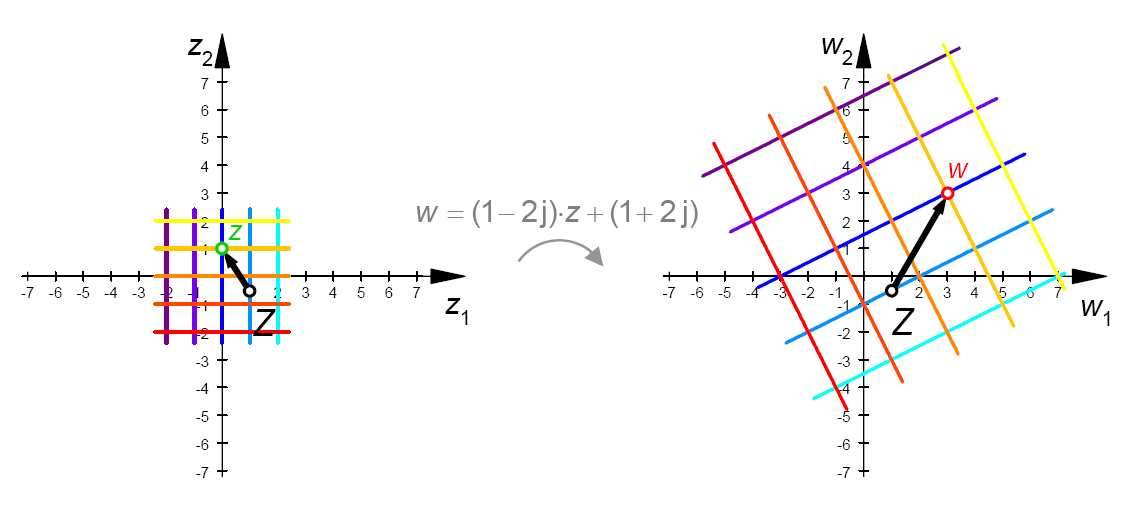
\includegraphics[width=8cm]{./bilder/LineareFunktion.png}
    \end{minipage}

\skriptsubsection{Quadratfunktion und Quadratwurzelfunktion}{45ff}
	\begin{minipage}{9cm}
    	$$ f : z \mapsto w = z^2 \qquad \qquad f : z \mapsto w = \sqrt{z} $$\\
		Bei der Quadratfunktion wird schon die rechte Hälfte der z-Ebene auf die ganze
		w-Ebene abgebildet (die Argumente werden verdoppelt). Daraus ergibt sich
		zwei bzw. mehrere Ebenen.
    \end{minipage}
	\hspace{2cm}
	\begin{minipage}{8cm}
    	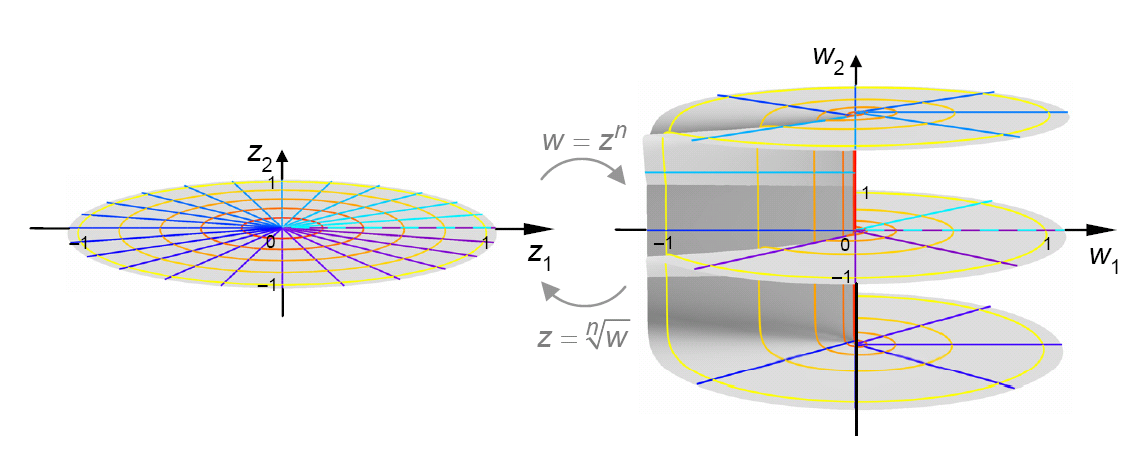
\includegraphics[width=8cm]{./bilder/RiemannischeFlaeche.png} 
    	Eine Riemanische Fläche 3.Grades
    \end{minipage}

\skriptsubsection{Kehrwertfunktion und Kreisspiegelung}{51ff}
	$$ f : z \mapsto w = \frac{1}{z}; \quad (\arg(w) = -\arg(z), |w| = \frac{1}{|z|})
	\qquad \qquad 
	\overline{f}: z \mapsto w = \frac{1}{\overline{z}};  \quad  
	(\arg(w) = \arg(z), |w| = \frac{1}{|z|}) $$\\
	Kreisspiegelung: Alle Punkte auf der z-Ebene werden am Einheitskreis gespiegelt.
	Geraden auf Kreise abgebildet und umgekehrt. Der Ursprungspunkt (0;0) wird auf
	$ \infty $ abgebildet (auf allen Winkeln zwischen $0^o-360^o$). Die
	Abbildungen sind
	im verallgemeinerten Sinn (Geraden sind Kreise mit unendlichem Radius)
	kreistreu. Ausserdem sind sie bis auf den Koordinatenursprung winkeltreu\\
	\begin{minipage}{9cm}
		\begin{tabbing}
        	xxxxxxxxxxxxxxxxxxxxxxx\=xxxxxxxxxxxxxxxxxxxxxxxx\kill
	        - Gerade durch 0 $\Longrightarrow$ \>Fixgerade (gleiche Gerade, aber
	        die \\ \>Punkte darauf sind anders verteilt)\\ \\
			- Gerade nicht durch 0 $\Longrightarrow$ Kreis durch 0\\ \\ \\ \\ \\ \\ \\ \\
			- Kreis nicht durch 0 $\Longrightarrow$ \>Spiegelung des Kreises\\ \> an dem
			Einheitskreis\\ \\
			- Kreis durch 0 $\Longrightarrow$\>Gerade nicht durch 0
        \end{tabbing}
	\end{minipage}
	\hspace{2cm}
	\begin{minipage}{6cm}
		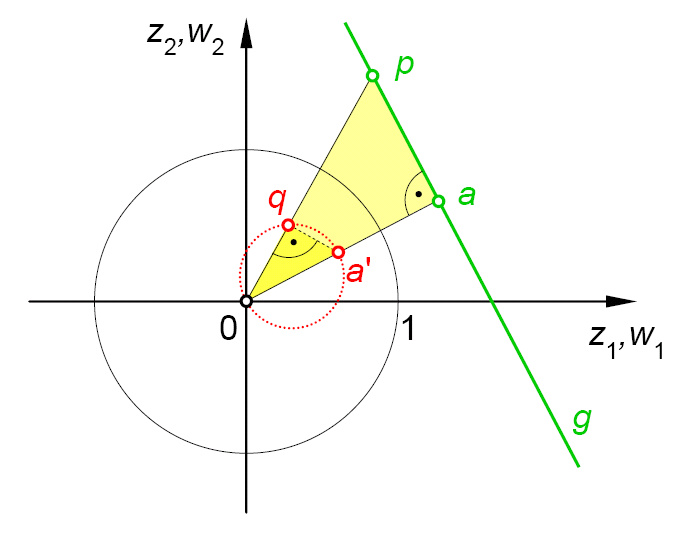
\includegraphics[width=6cm]{./bilder/GeradeKreisspiegelung.png} 
    	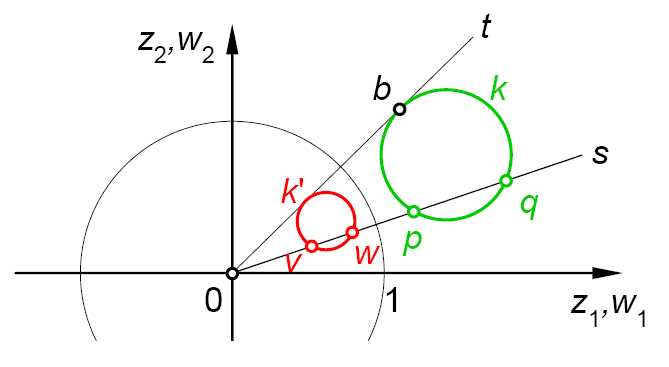
\includegraphics[width=6cm]{./bilder/KreisKreisspiegelung.png}
    \end{minipage}

\skriptsubsection{Möbiustransformation}{57ff}
	\begin{minipage}{10cm}
		$$ f : z \mapsto w = f(z) = \frac{az + b}{cz + d}$$
		$$(a, b, c, d \in 
		\mathbb{C} \text{ mit } c \neq 0 \text{ und } ad - bc \neq 0) $$
		Die Möbiustransformation ist eine Verkettung einer linearen Funktion, der Kehrwertfunktion und einer weiteren linearen Funktion. \\
		Diese Transformationen sind winkel- und kreistreu. Die Umkehrfunktion ergibt wieder eine Möbiustransformation. \\
		Eigentlich besitzt diese Funktion nur drei Parameter da man den Bruch
		$\frac{az + b}{cz + d}$ stets so kürzen kann dass einer der vier Parameter 1
		ist. Durch die 3 Freiheitsgrade kann man unterschiedlichste kriterien
		vorgeben und damit komplizierte Umformungen machen, wie im Bild gezeigt wird:
	
	\end{minipage}
	\hspace{2cm}
	\begin{minipage}{7cm}
		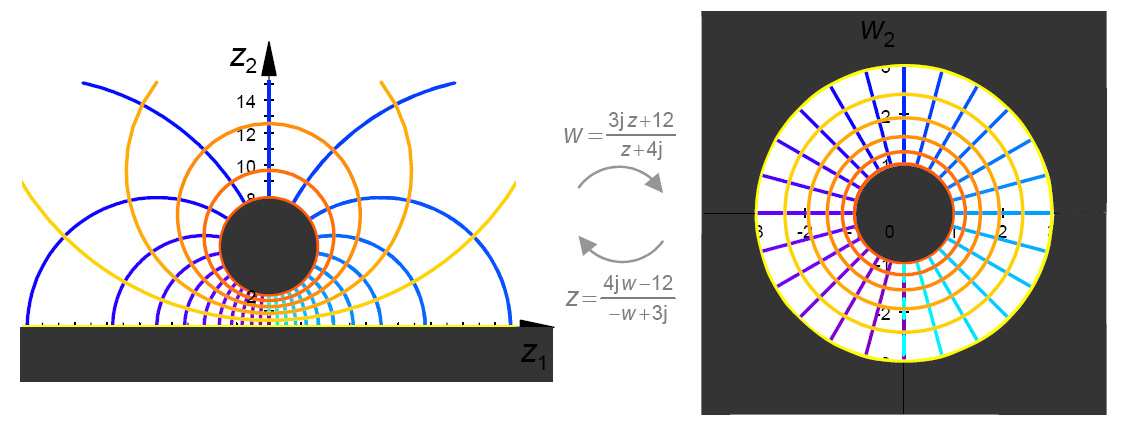
\includegraphics[width=7cm]{./bilder/Moebiustransformation.png} 
	\end{minipage}

\skriptsubsection{Joukowski-Funktion}{60ff}
	\begin{minipage}{10cm}
		$$ f : z \mapsto w = z + \frac{1}{z}  $$
		Die Funktion ist winkeltreu bis auf $\pm$2\\
		Wenn man einen Kreis, der nicht ganz im Zentrum steht transformiert ergibt
		sich ein Flügelprofil
	\end{minipage}
	\hspace{2cm}
	\begin{minipage}{7cm}
		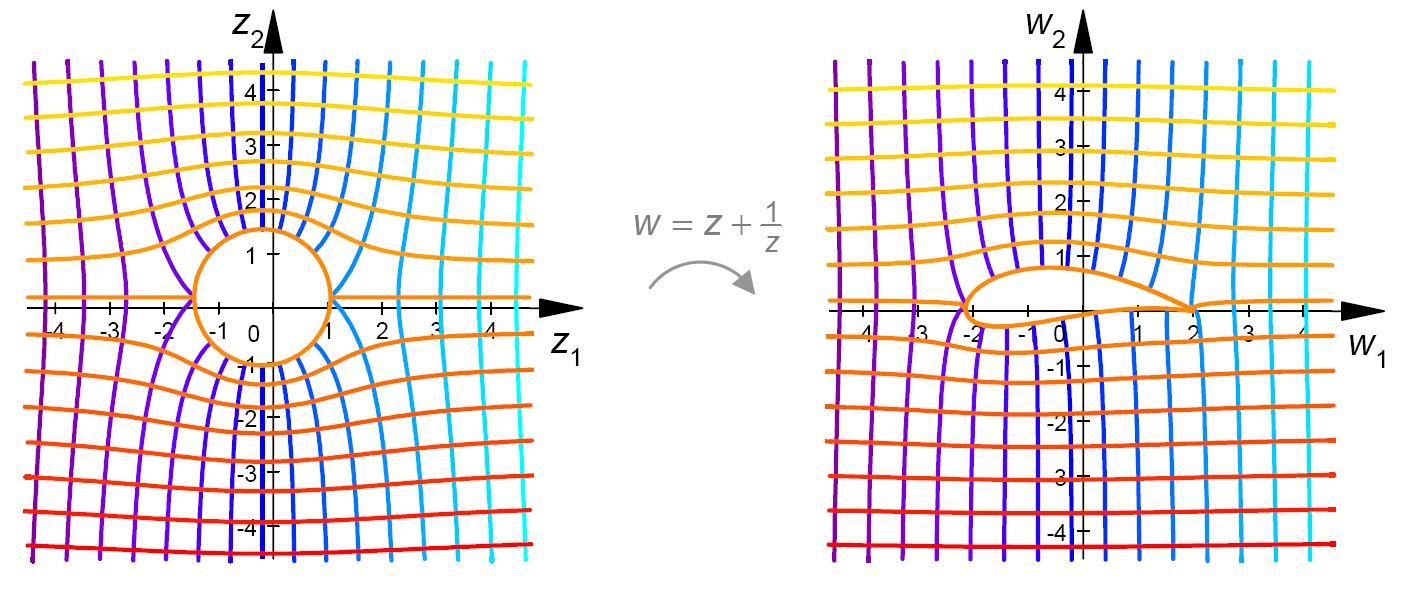
\includegraphics[width=7cm]{./bilder/joukowskiFunktion.png} 

	\end{minipage}
\skriptsubsection{Exponentialfunktion}{64ff} 
	\begin{minipage}{9cm}
		$$ f : z \mapsto w = e^z $$
		Waagrechte Gitternetzlinen gehen gemäss der obigen Gleichung in Strahlen
		über, die im Koordinatenursprung beginnen, senktrechte Gitternetzlinien in
		Kreise um den Koordinatenursprung. Die e$^z$-Funktion ist periodisch, deshalb
		braucht es eine Riemansche Fläche\\ \\
		Mit dieser Funktion kann man das Feld bei den Rändern des Plattenkondensator
		berechnen 
	\end{minipage}
	\hspace{2cm}
	\begin{minipage}{7cm}
		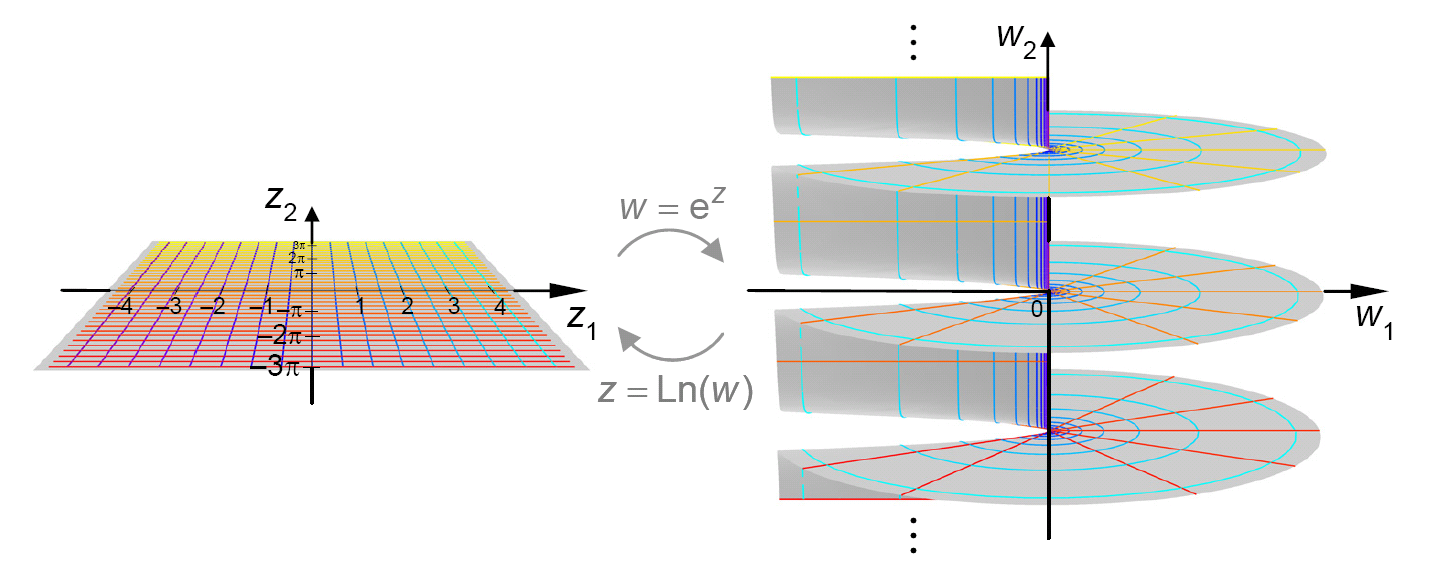
\includegraphics[width=7cm]{./bilder/ehochz.png} 
		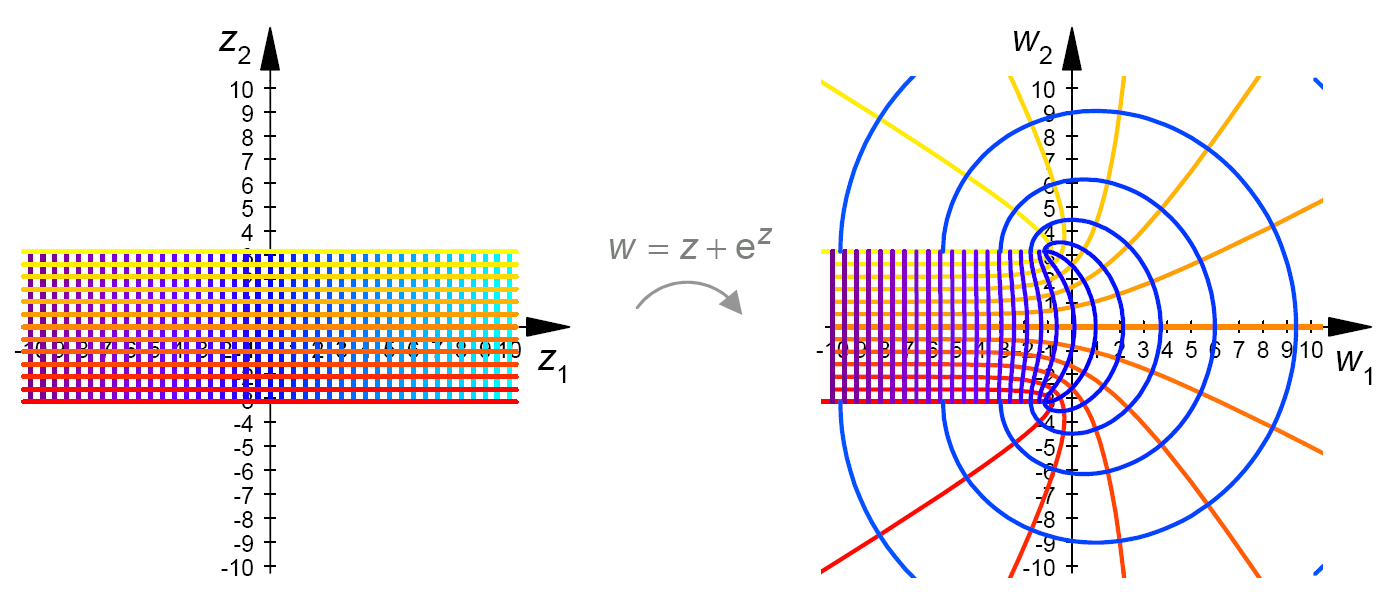
\includegraphics[width=8cm]{./bilder/plattenkondensator.png} 		
	\end{minipage}

\skriptsubsection{Sinus-Funktion}{67f}
	 \begin{minipage}{10cm}
		$$ f : z \mapsto w = \sin(z) $$    
		Die Sinusfunktion ist ausser bei den Punkten $z = \frac{\pi}{2}+ k\pi (k \in
		\mathbb{Z}))$ winkeltreu
	\end{minipage}
	\hspace{2cm}
	\begin{minipage}{7cm}
		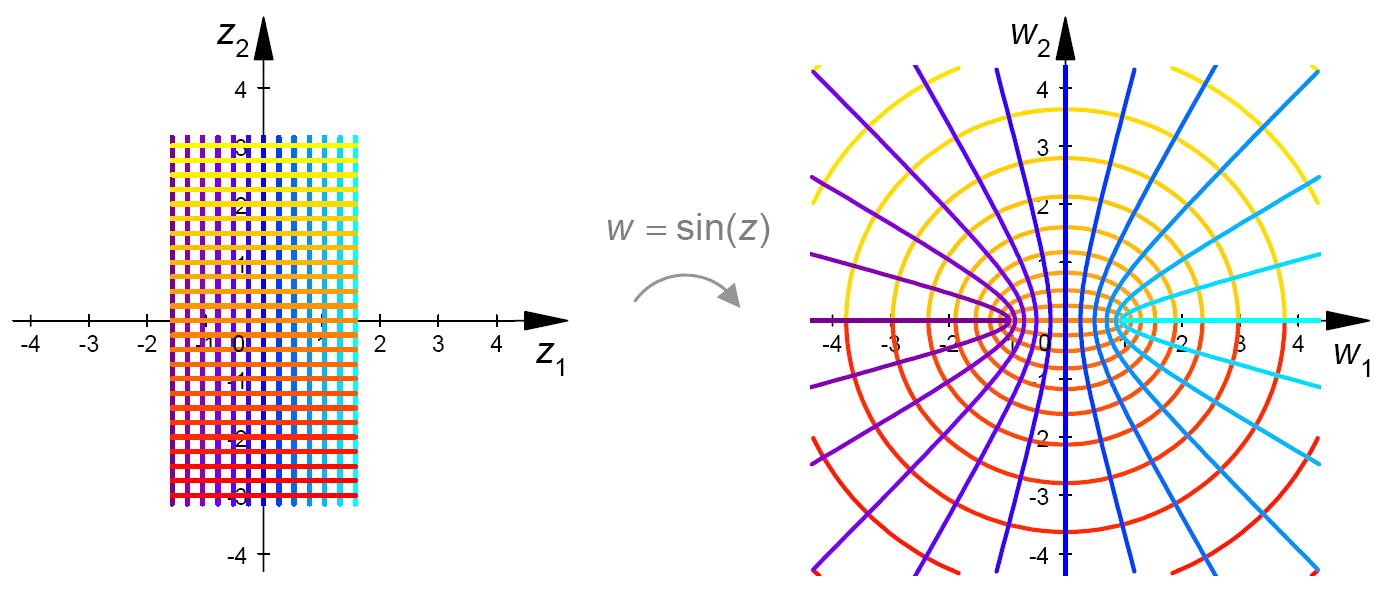
\includegraphics[width=7cm]{./bilder/sinus.png} 
	
	\end{minipage}
 
\subsection{Kreisgleichung}
Die Lösungen von z bilden einen Kreis in der mit dem Radius $r$ um den Mittelpunkt $M=(m_x, m_y) \Rightarrow m=m_x + j m_y$. \\
$$|z-m| = r; \qquad 
(z-m)(\overline{z} - \overline{m}) = r^2; \qquad 
z\overline{z} - \overline{m}z - m\overline{z} + m\overline{m} = r^2$$
$$ \text{Parameterform: } f(t) = m + r \cdot e^{jt}, \quad \text{mit } (0 \leq t \leq 2 \pi) $$


\newpage
\skriptsection{Fourierreihen}{67ff}
    \skriptsubsection{Orthogonalitätsbeziehungen der Basisfunktionen}{75}
        \begin{tabular}{lll}
            $\int\limits_0^T \cos(n\omega t)\cdot \cos(m\omega t)dt=
            \begin{cases}
            T,\ n=m=0\\
            \frac{T}{2},\ n=m>0\\ 
            0,\ n\neq m\\
            \end{cases}$ &
            $\int\limits_0^T \sin(n\omega t)\cdot \sin(m\omega t)dt=
            \begin{cases}
            \frac{T}{2},\ n=m\\
            0,\ n\neq m\\
            \end{cases}$&
            $\int\limits_0^T \cos(n\omega t)\cdot \sin(m\omega t)dt=0$
        \end{tabular}
	\skriptsubsection{Allgemeine Form}{79}
		Eine periodische Funktion f mit Periode $T>0$, lässt sich durch eine Reihe von
		Sinus- und Kosinusfunktionen darstellen, deren Frequenzen ganzzahlige 
		Vielfache der Grundfrequenz $\omega = 2\pi / T$ sind:
		$$ f(t)=\frac{a_0}{2} + \sum_{n=1}^\infty (a_n \cdot \cos(n \omega t) + b_n
		\cdot \sin(n\omega t))$$
		Die Koeffizienten der Entwicklung von $f(t)$ sind:
		$$ a_n=\frac{2}{T}\int_{0}^{T} f(t) \cdot \cos(n\omega t)\, \mathrm{d}t \quad (n=0,1,2,3,\ldots)
		 \qquad \qquad b_n=\frac{2}{T}\int_{0}^{T} f(t) \cdot \sin(n\omega t)\,
		 \mathrm{d}t \quad (n=1,2,3,\ldots) $$
		Der erste Summand der Reihe $a_0/2$ ist der Gleichstromanteil (Mittelwert) von
		$f(t)$ im Intervall $(0,T)$

	\skriptsubsection{Komplexwertige Darstellung der Fourierreihen}{95ff}
		$$f(t) = \sum\limits_{k = -\infty}^{\infty} c_k \cdot e^{j k \omega t} \qquad \text{mit} \qquad c_n=\overline{c_{-n}}=\frac{1}{T}\int_0^T{f(t)\cdot e^{-jn\omega t}dt}$$
		\subsubsection{Umrechnungsformeln}
			$$c_n=\overline{c_{-n}}=\frac{a_n-jb_n}{2} (n=0,1,2,3,\ldots\text{ wobei }b_0=0)\qquad
			\left.
			\begin{array}{l} 
				a_n=2 \cdot \text{Re}(c_n)\\
				b_n=-2 \cdot \text{Im}(c_n)
			\end{array}
		    \right\} 
		    \quad
			(n=0,1,2,3,\ldots, b_0 = 0)$$

	\skriptsubsection{LTI-Systeme}{72} 
	    \subsubsection{Linear}
	    \begin{tabular}{llll}
            \textbf{Aus}: &
            $f(t)\to \fbox{S}\to F(t)$ &
            und &
            $g(t)\to \fbox{S}\to G(t)$ \\
            \textbf{folgt} &
            $f(t)+g(t)\to \fbox{S}\to F(t)+G(t)$ &
            und &
            $r\cdot f(t)\to\fbox{S}\to r\cdot F(t)$ \\
        \end{tabular}
        \subsubsection{Zeitinvarianz}
        \begin{tabular}{llll}
            \textbf{Aus} &
            $f(t)\to \fbox{S}\to F(t)$ &
            \textbf{folgt} &
            $f(t+t_0)\to \fbox{S}\to F(t+t_0)$\\
        \end{tabular}
	\skriptsubsection{Sätze zur Berechnung der Koeffizienten}{80ff}
		\skriptsubsubsection{Symmetrie}{80f}
		\begin{tabular}{ll}
   			Falls $f(t)$ \textbf{gerade} ($ f(-t)=f(t) $) ist 
   			& $\quad \Longrightarrow \quad 
			b_n = 0, \quad a_n = \frac{4}{T} \int\limits_0^{\frac{T}{2}} f(t) \cdot
			\cos(n \omega t) \mathrm{d}t$ \\
			Falls $f(t)$ \textbf{ungerade} ($ f(-t)=-f(t) $) ist
			&$\quad \Longrightarrow \quad a_n = 0, \quad b_n =  \frac{4}{T} 
			\int\limits_0^{\frac{T}{2}} f(t) \cdot \sin(n \omega t) \mathrm{d}t$
      	\end{tabular}
			 
		\skriptsubsubsection{Linearität}{82}
			$h(t) = r \cdot f(t) + s \cdot g(t) \quad \Longrightarrow \quad a_n^{(h)} = r \cdot
			a_n^{(f)} + s \cdot a_n^{(g)}, \quad b_n^{(h)} = r \cdot b_n^{(f)} + s \cdot b_n^{(g)}$
			
		\skriptsubsubsection{Zeitstreckung/-stauchung ("Ahnlichkeit)}{83}
			$g(t) = f(r \cdot t) $ (mit $ 0 < r \in \mathbb{R}$ ) $\quad \Longrightarrow\quad  
			a_n^{(g)} = a_n^{(f)}, \quad b_n^{(g)} = b_n^{(f)} $ \quad $T^{(g)} = \frac{T^{(f)}}{r}$.
			
		\skriptsubsubsection{Zeitverschiebung}{84} 
		\label{Fourier_Zeitverschiebung}
		$g(t)=f(t+t_0)$
		$\qquad
		\begin{array}{l}
           a_n^{(g)}=\cos(n\omega t_0)\cdot a_n^{(f)}+\sin(n\omega t_0)\cdot b_n^{(f)}\\
           b_n^{(g)}=-\sin(n\omega t_0)\cdot a_n^{(f)}+\cos(n\omega t_0)\cdot b_n^{(f)}\\
           c_n^{(g)}=e^{jk \omega t_o} \cdot c_k^{(f)}
        \end{array}$
        $\quad
		\begin{array}{l}
           (n=0,1,2,\ldots)\\
           (n=1,2,3,\ldots)\\
           (k \in \mathbb{Z})
        \end{array}$ \\
		
\skriptsubsection{Integral und Differential}{88}
Falls die T-periodische Funktion $f$ (auf ganz $\mathbb{R}$) zweimal stetig differenzierbar ist und die Fourierkoeffizienten $a_n$ und $b_n$ besitzt, so gilt:
$$ f'(t) = \sum\limits_{n=1}^{\infty} [b_n n \omega \cdot \cos{(n \omega t)} - a_n n \omega \cdot \sin{(n \omega t)}]
\qquad \qquad \int\limits_0^t f(\tau) d\tau = \sum\limits_{n=1}^{\infty} \frac{b_n}{n \omega} + 
\frac{a_0}{2} t + \sum\limits_{n=1}^{\infty}
[\frac{a_n}{n \omega} \cdot \sin{(n \omega t)} - \frac{b_n}{n \omega} \cdot \cos{(n \omega t)}] $$

\skriptsubsection{Gibbs'sches Phänomen}{92f}
Die Fourier-Reihen schwingen bei Unstetigkeitsstellen über. Die Höhe des
Überschwingers lässt sich so berechnen:

\begin{figure}[htbp]
	\begin{minipage}[b]{8cm}
$$\frac{1}{\pi}\int\limits_0^\pi \frac{\sin t}{t}\, \mathrm dt - \frac{1}{2} =
0{,}089490\dots$$ \\
	\end{minipage}
	\begin{minipage}[b]{8cm}
		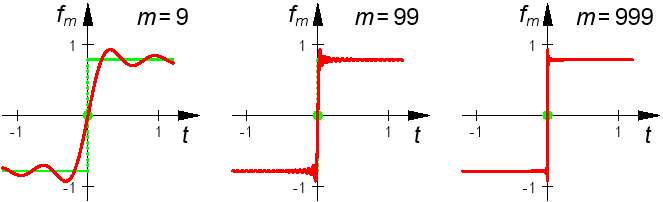
\includegraphics[width=8cm]{./bilder/gibssches_phaenomen.png}  
	\end{minipage}
\end{figure}

\skriptsubsection{Frequenz-, Amplituden- und Phasengang}{72}
$ \text{Frequenzgang eines Systems: } H(\omega) = A(\omega) \cdot e^{j \Phi(\omega)} \qquad 
\text{ Amplitudengang: } A(\omega) = |H(\omega)| \qquad \text{ Phasengang } \Phi(\omega) = arg[H(\omega)] $ \\ \\
Die komplexe Funktion $H(\omega)$ der reellwertigen Frequenz $\omega$ enthält zugleich die Informationen über 
die Veränderung der Amplitude und der Phasenverschiebung des Systems S bei der betrachteten Frequenz $\omega$.
$$f(t) = Im[z(t)] \to \fbox{S}\to F(t) = Im[z(t) \cdot H(\omega)] \qquad \text{ oder } 
\qquad f(t) = Re[z(t)] \to \fbox{S}\to F(t) = Re[z(t) \cdot H(\omega)]$$
Je nach Eingangssignal wird der Real- oder der Imaginärteil behandelt: 
$ f(t) = 
		\left\{
		\begin{array}{l}
           sin(n t) = Im[e^{j \cdot n t}]\\
           cos(n t) = Re[e^{j \cdot n t}]
        \end{array}
		\right\}
\Longrightarrow
z(t) = e^{j \cdot n t}
$ \\

Somit kann die Antwort des Systems mittels einer komplexen Multiplikation mit der Hilfsfunktion $z(t)$ berechnet werden.


\begin{center}
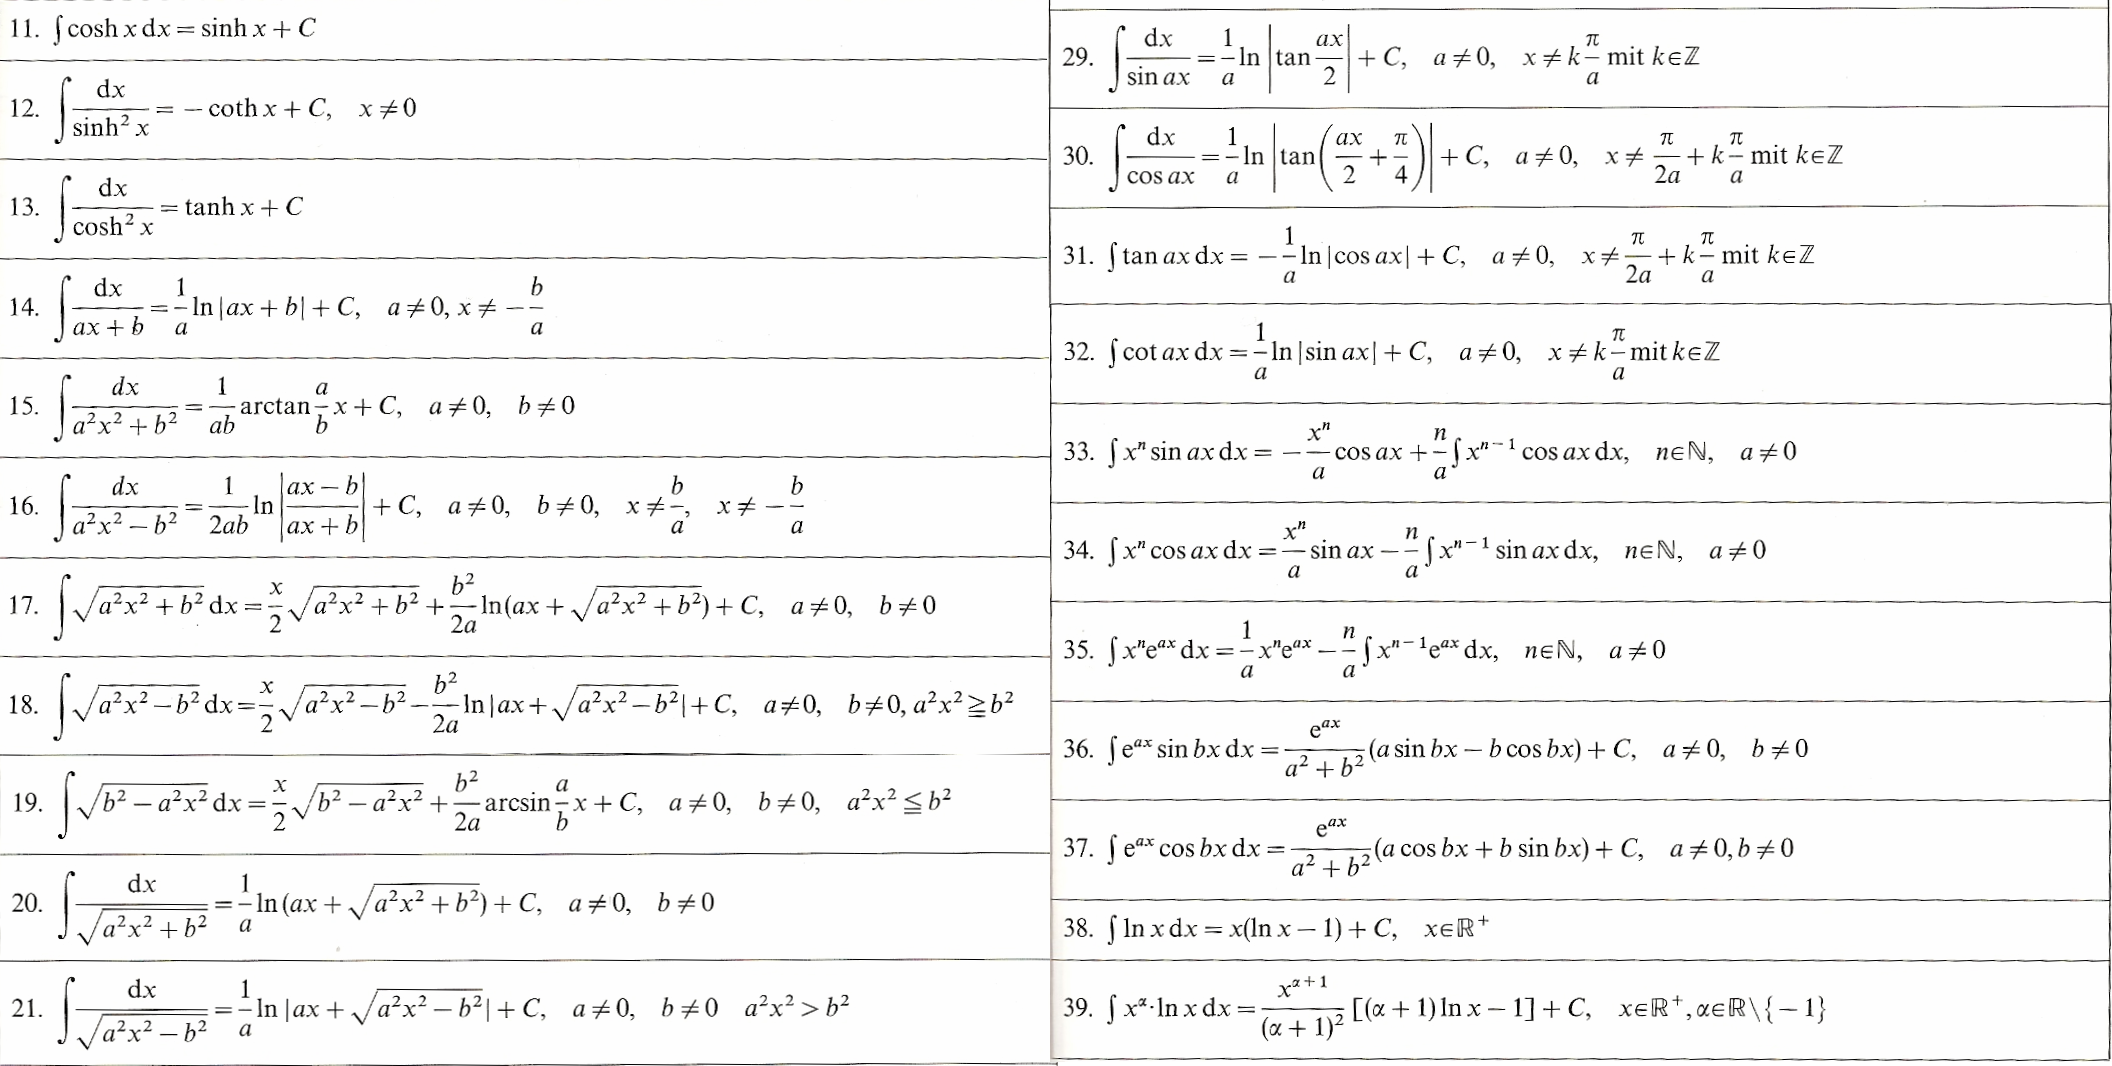
\includegraphics[width=18cm]{./bilder/integral2.png}
\end{center}




\newpage
\skriptsection{Spektren}{103}
\skriptsubsection{Spektraldarstellungen}{103ff} 

\begin{figure}[htbp]
	\centering
	\begin{minipage}[b]{5.5cm}
		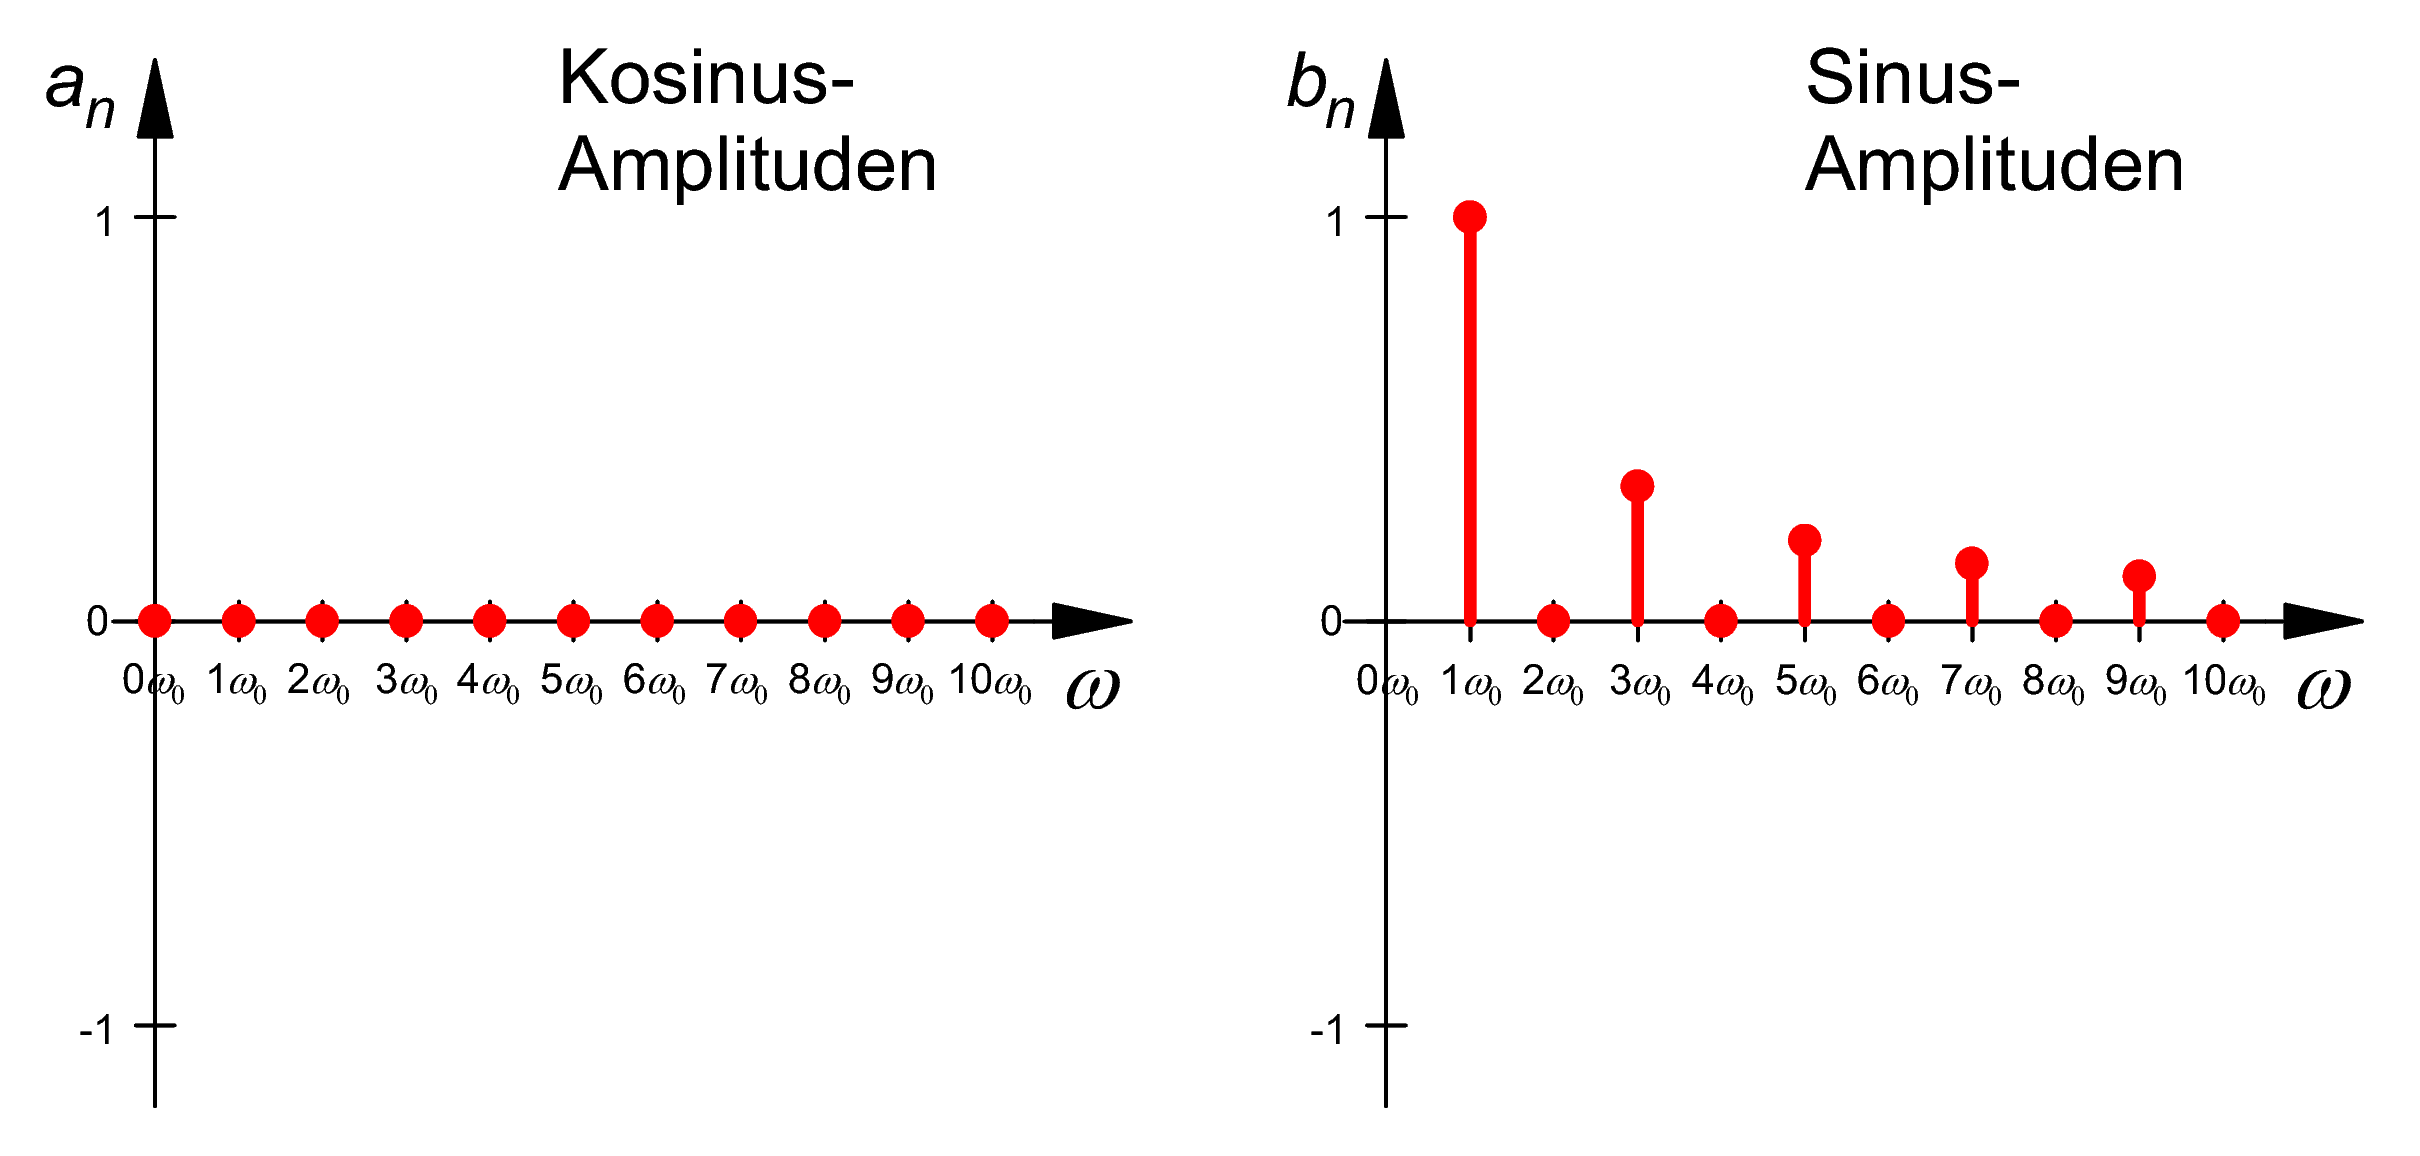
\includegraphics[width=5.5cm]{./bilder/spektren_cossin.png}
		\caption{Kosinus- und Sinusamplitudendiagramm} 
	\end{minipage}
	\hspace{1cm}
	\begin{minipage}[b]{5.5cm}
		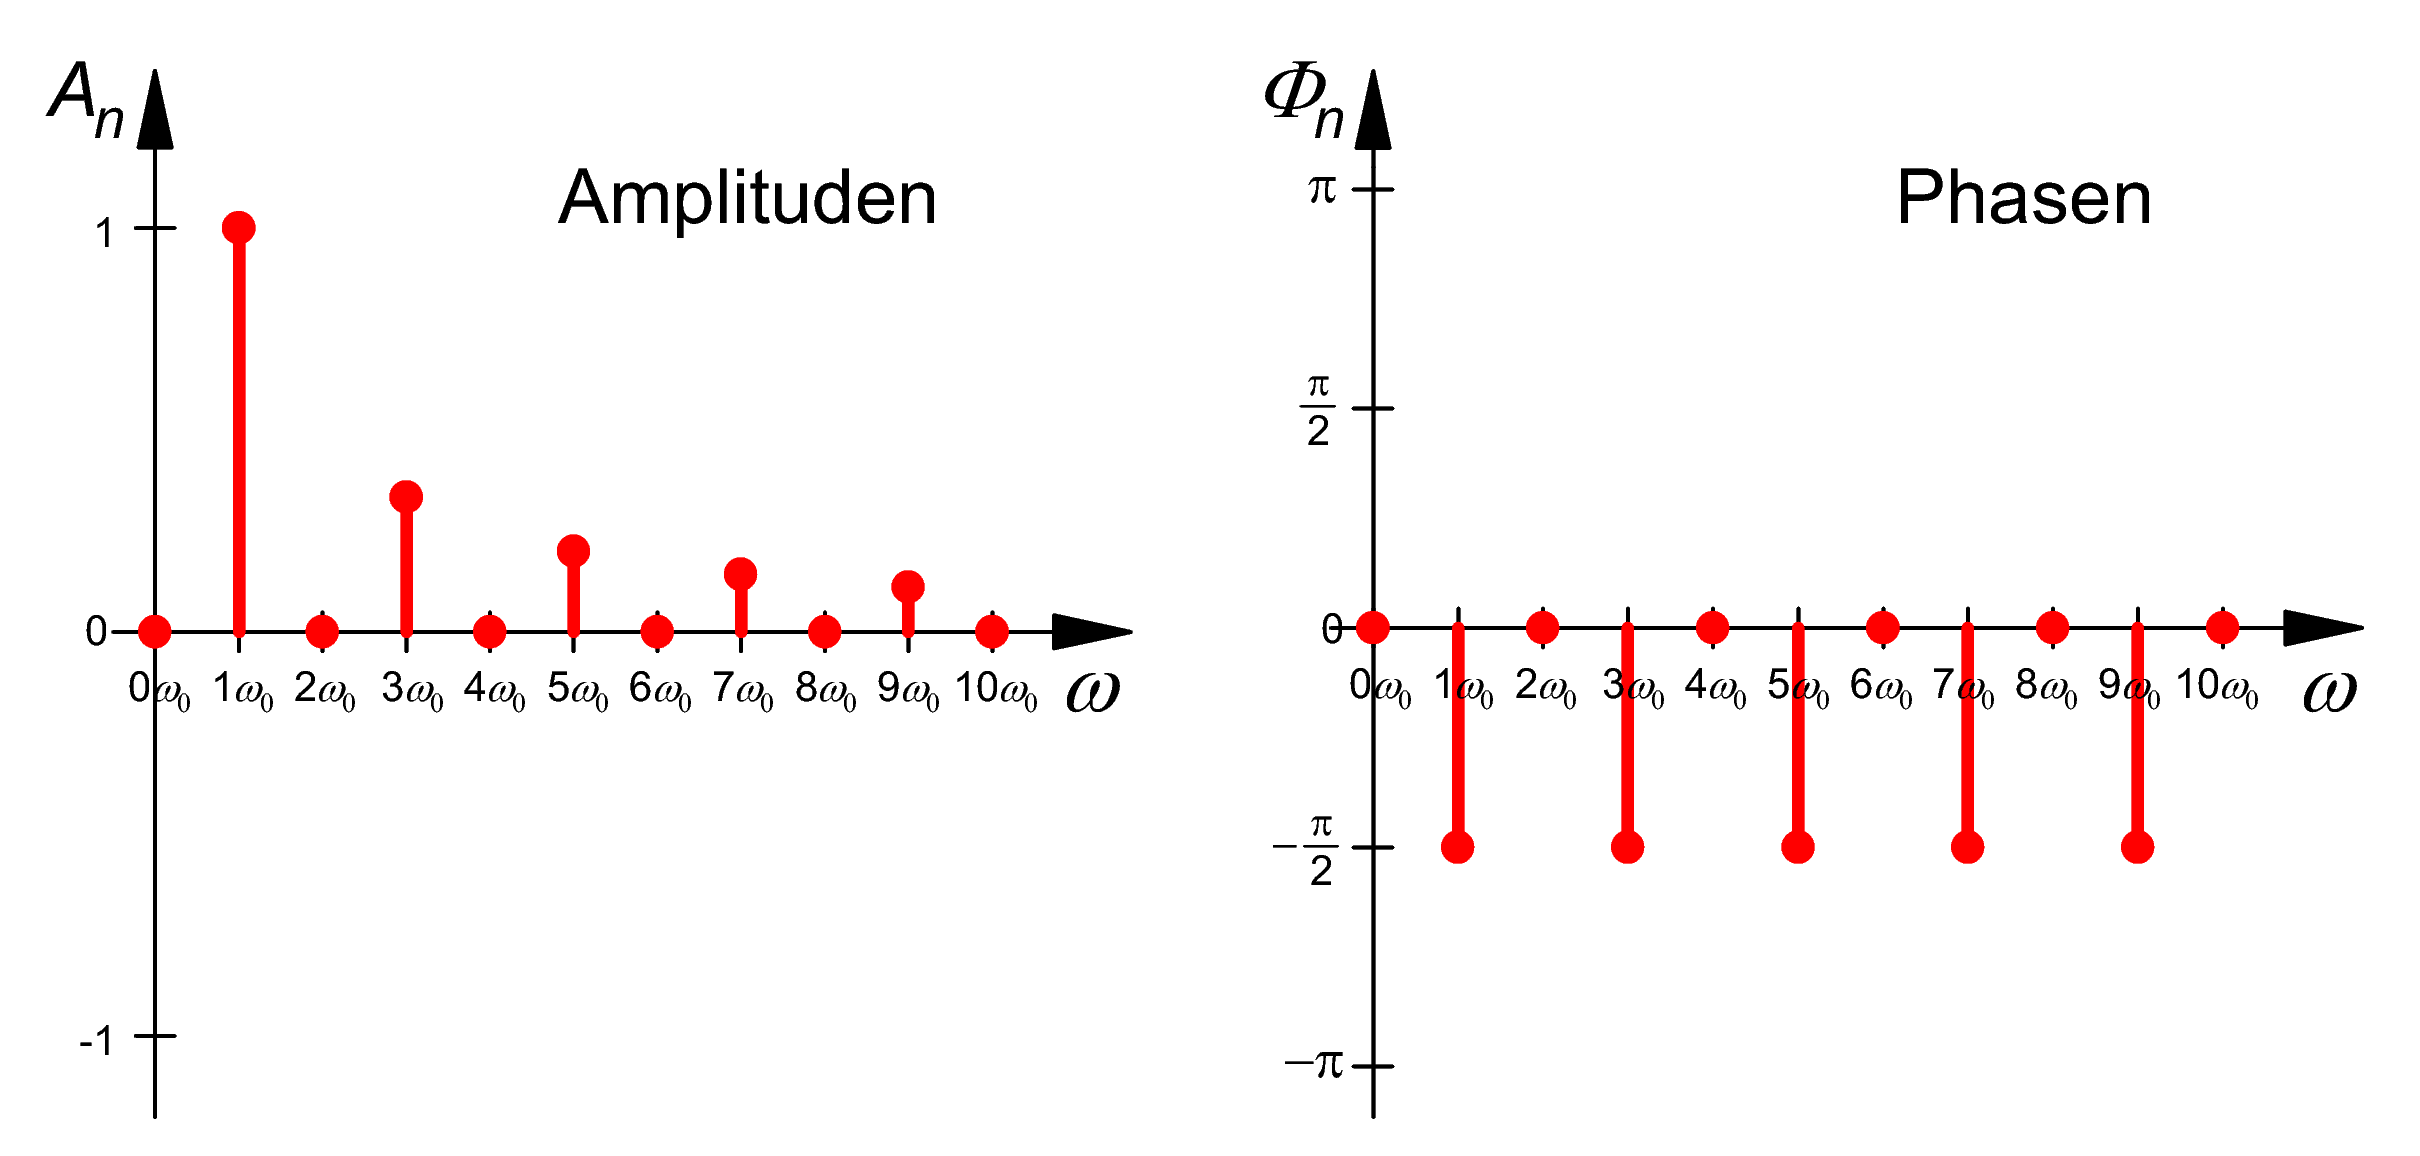
\includegraphics[width=5.5cm]{./bilder/spektren_einseitig.png} 
		\caption{Einseitiges Amplituden-/Phasendiagramm} 
	\end{minipage}
	\hspace{1cm}
	\begin{minipage}[b]{5.5cm}
		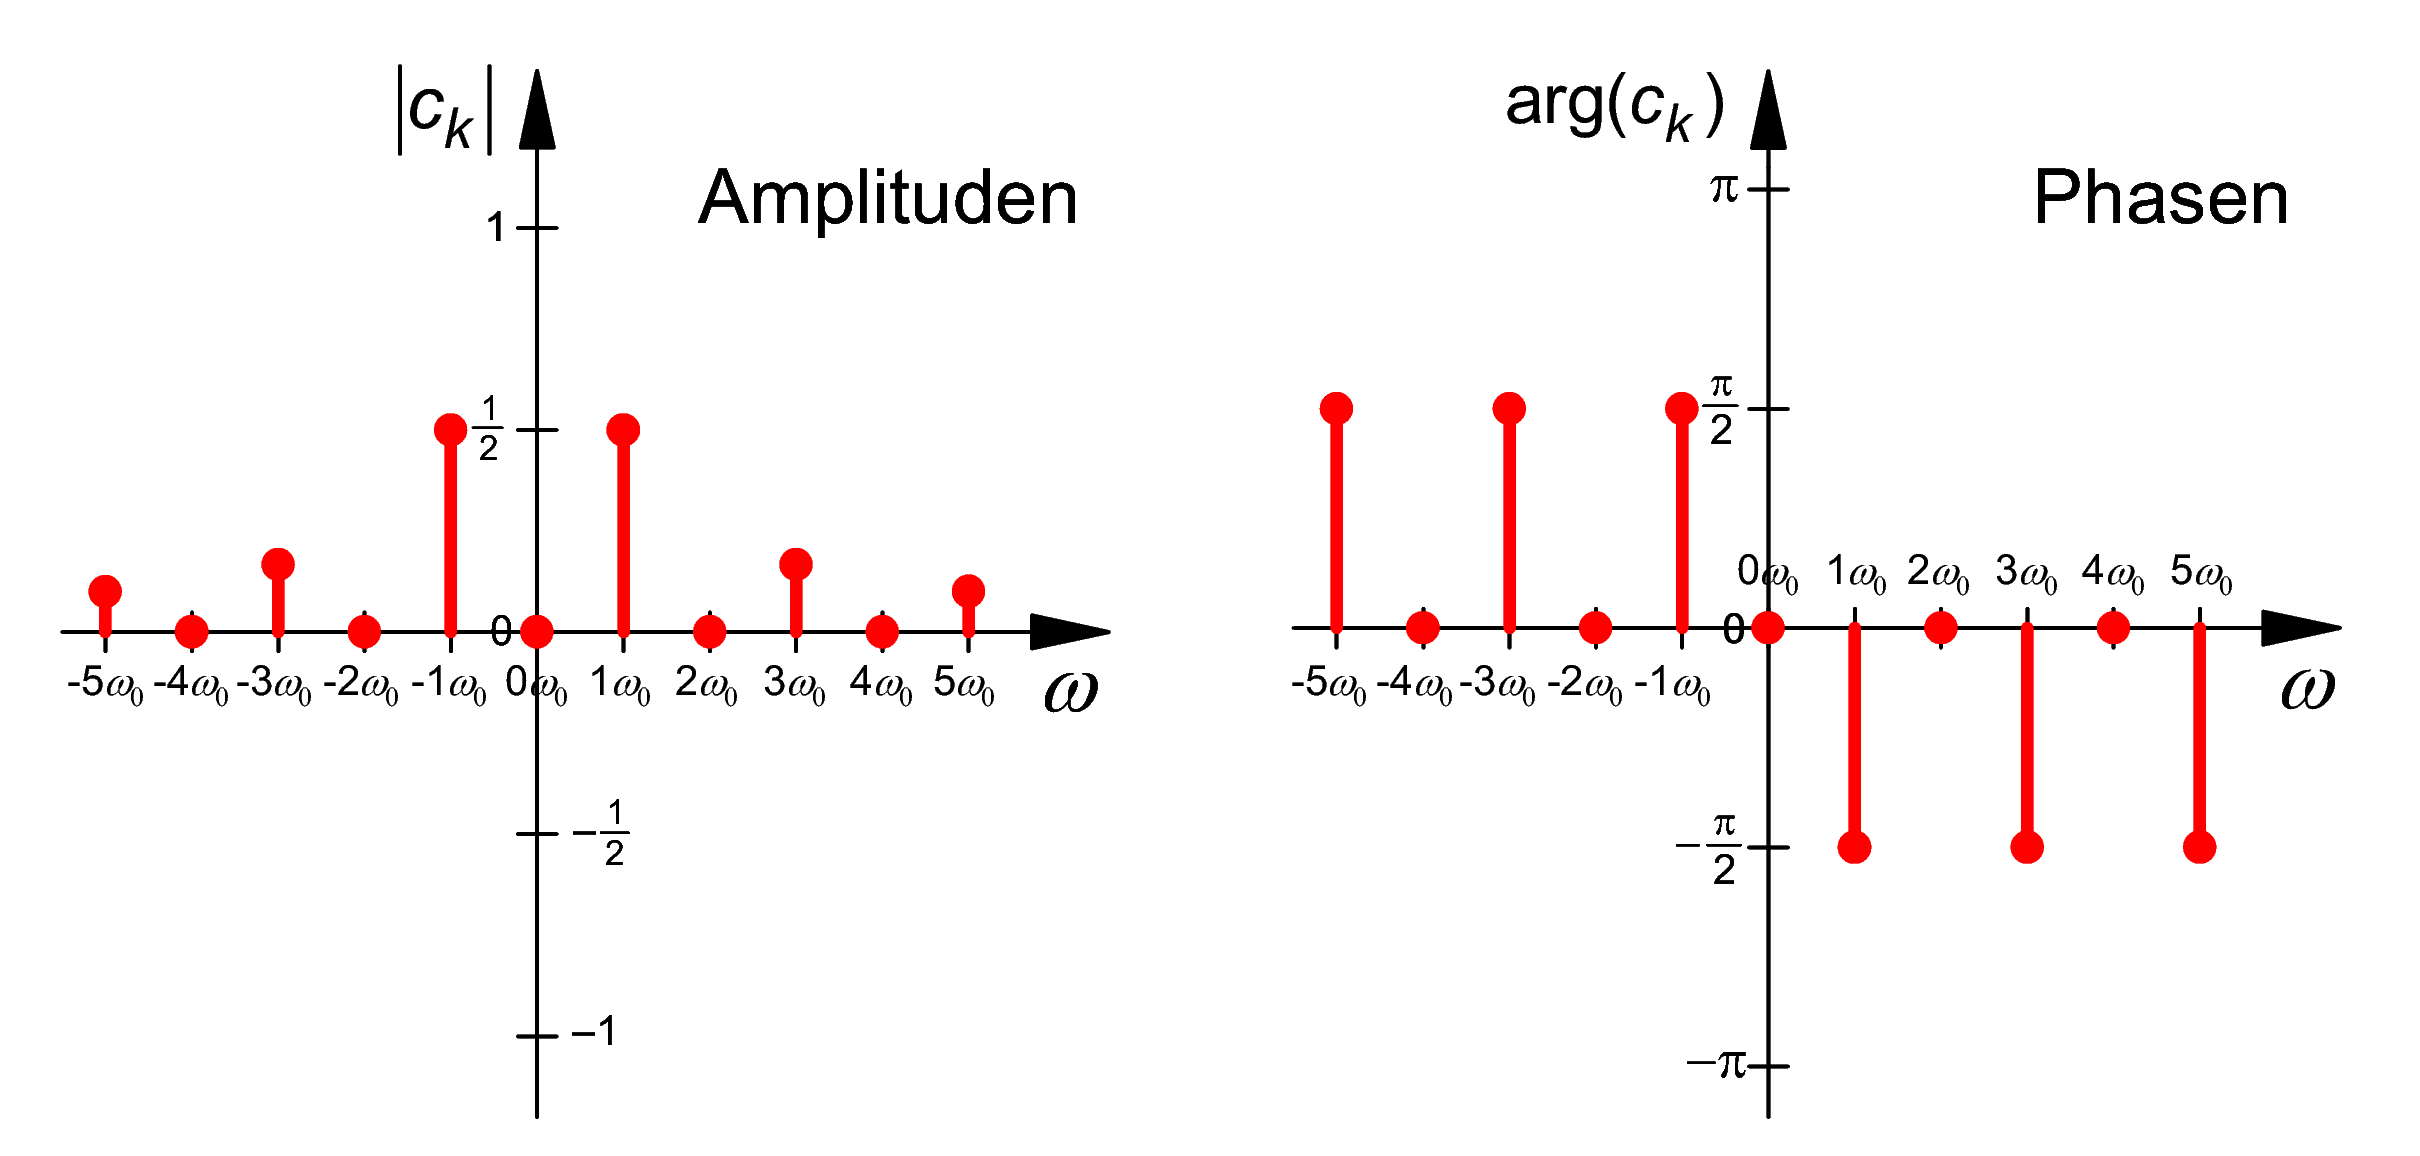
\includegraphics[width=5.5cm]{./bilder/spektren_zweiseitig.png} 
		\caption{Zweiseitiges Amplituden-/Phasendiagramm} 
	\end{minipage}
\end{figure}

\subsubsection{(1) Kosinus- und Sinusamplitudendiagramm} 
Reelle Fourierkoeffizienten ($a_n, b_n$) können direkt abgelesen werden. 
Bei einer Phasenverschiebung ändern sich jedoch die Koeffizienten grafisch nicht nachvollziehbar. \\
Diese Darstellung hat gegenüber den anderen zwei mehr Nachteile und wird daher eher selten genutzt.

\subsubsection{(2) Einseitiges Amplituden-/Phasendiagramm} 
$A_n = |a_n - j \cdot b_n| = \sqrt{a_n^2 + b_n^2}$ \text{ oder } $A_n = 2 \cdot |c_n| \qquad$
$\Phi_n = \arg(a_n - j \cdot b_n) \text{ oder } \Phi_n = \arg(c_n) $ \\
Spezialfall $n=0 \Rightarrow A_0 = |\frac{a_0}{2}| \text{ und } \Phi_0 = \left\{
		\begin{array}{l} 
			0, \quad a_0 \geq 0\\
			\pi, \quad a_0 < 0  
		\end{array}
	    \right. $

\subsubsection{(3) Zweiseitiges Amplituden-/Phasendiagramm (komplexes Spektrum)} 
Amplitudendiagramm ist achsensymmetrisch wegen $ c_n=\overline{c_{-n}} $. Phasendiagramm ist punktsymmetrisch. \\
Ähnlichkeit mit Einseitigem: $|c_k| = \frac{1}{2}A_k $ und $\arg(c_k) = \Phi_k$ für alle $ n \geq 0$.

\skriptsubsection{Spezialfälle}{106}
\begin{tabular}{ll}
	Funktion f gerade 
	& (1) Sinusamplitudendiagramm überall 0 \\
	& (2,3) Phasendiagramm enthält nur die Werte $0$ und $\pi$ \\
	Funktion f ungerade
	& (1) Kosinusamplitudendiagramm überall 0 \\
	& (2,3) Phasendiagramm enthält nur die Werte $\pm \frac{\pi}{2}$ (oder $0$ falls Amplitudenwert $=0$) \\
	"Ahnlichkeit $g(t) = f(r \cdot t) $
	& (1,2,3) Das Spektrum von $g$ ist das horizontal mit den Faktor $r$ gestreckte Spektrum vom $f$. \\
	Zeitverschiebung $g(t) = f(t + t_0) $
	& (1) \verweis{Fourier_Zeitverschiebung}{Zeitverschiebung} \\
	& (2,3) Amplitudendiagramme sind identisch. \\
	& (2,3) Phasendiagramme: Die Sälule der Frequenz $k \omega_0$ wächst um $k\omega_0 t_0$. \\
	Weisses Rauschen
	& "Uberlagerung von Schwingungen aller möglichen Frequenzen \\
	& mit gleichen Amplituden und zufälligen Phasen. 

\end{tabular}

\begin{center}
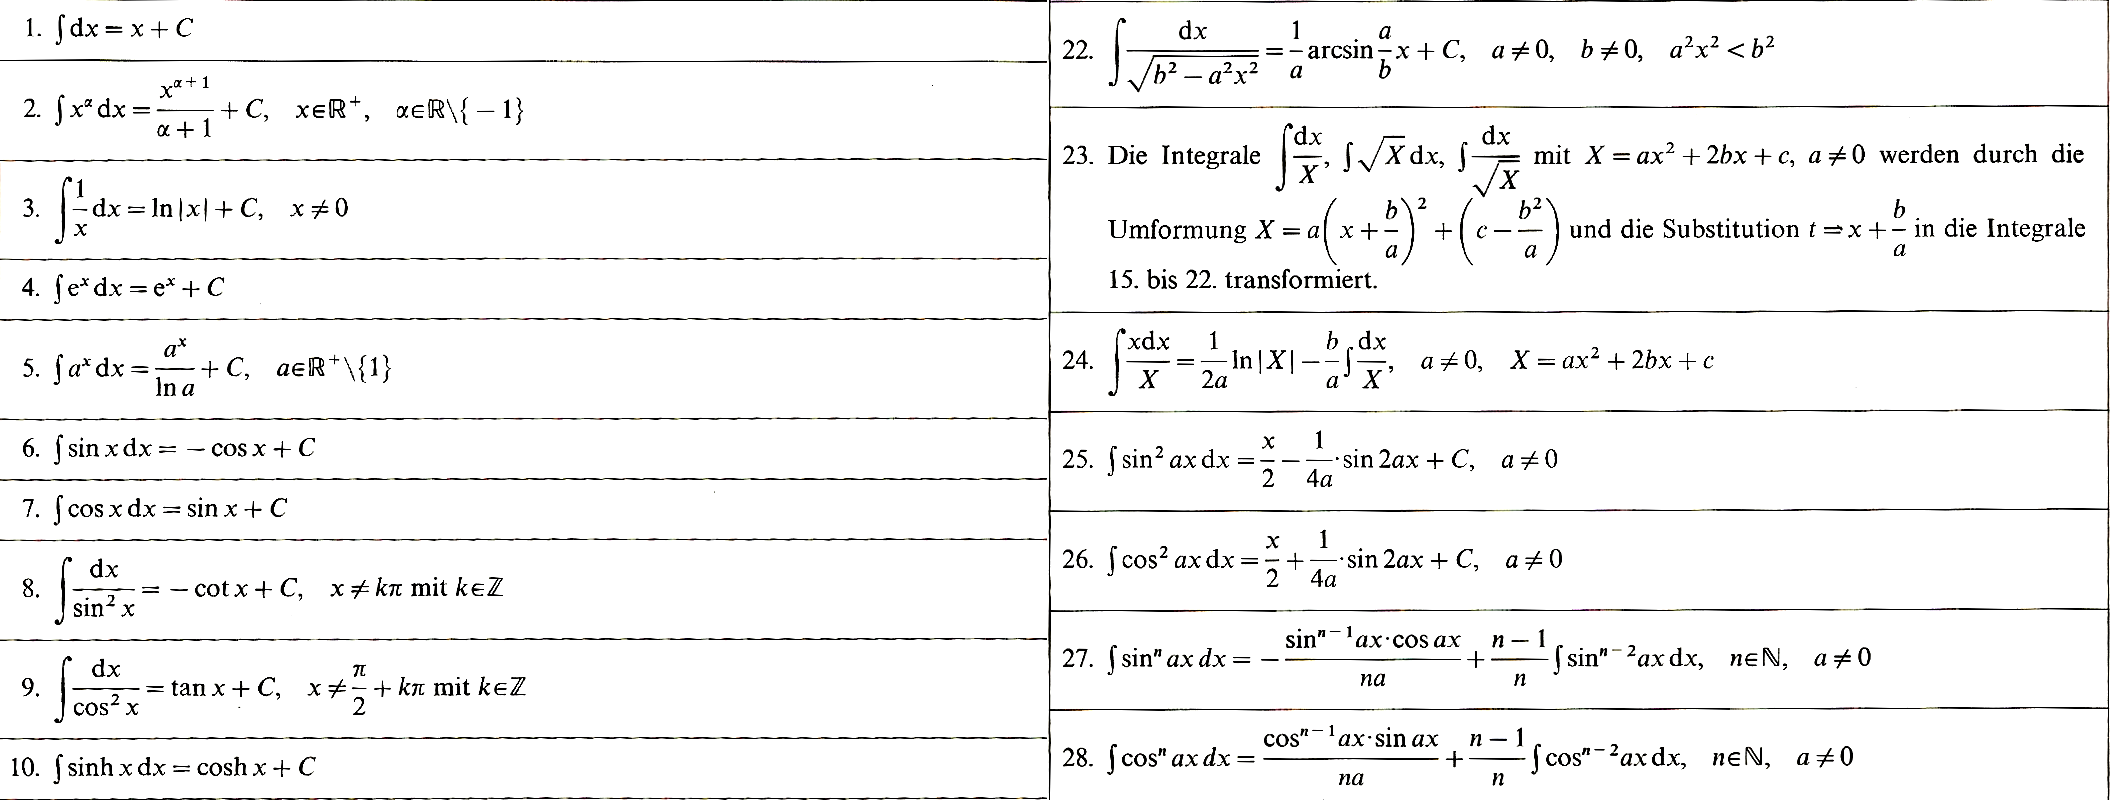
\includegraphics[width=18cm]{./bilder/integral1.png}
\end{center}





\newpage 
\skriptsection{DFT - Diskrete Fourier Transformation}{109}
\subsection{Definitionen}
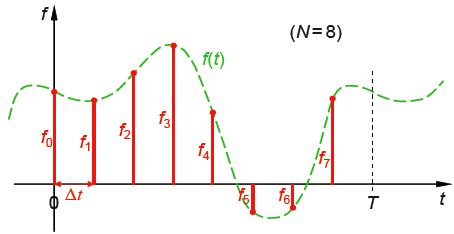
\includegraphics[width=5cm]{./bilder/abtastung.png}

\subsubsection{Diskrete komplexe Fourierkoeffizienten}
$\hat{c_k}$ sind die diskreten Fourierkoeffizienten die zu den (reellen
Abtastwerten $f_0, f_1,\ldots,f_{N-1}$) gehören\\
$$\hat{c_k}=\frac{1}{N}\sum\limits_{n=0}^{N-1}f_n\cdot e^{-\frac{2\pi j}{N}\cdot
kn}$$
Kompakte Darstellung mit der Matrix W:
$\begin{pmatrix}
 \hat{c_0}\\\hat{c_1}\\\hat{c_2}\\\hat{c_3}
\end{pmatrix}$
$=\frac{1}{N}$
$\begin{pmatrix}
 w^0w^0w^0w^0\\w^0w^1w^2w^3\\w^0w^2w^4w^6\\w^0w^3w^6w^9
\end{pmatrix}$
$\cdot$
$\begin{pmatrix}
 f_0\\f_1\\f_2\\f_3
\end{pmatrix}$
wobei $w=e^{-\frac{2\pi j}{N}}$

\subsubsection{Rechenaufwand DFT / FFT}
Der Rechenaufwand für die DFT ist proportional zu $N^2$ 
hingegen ist er bei der Fast Fourier Transform (FFT) nur $N\cdot log(N)$.

\skriptsubsection{Eigenschaften der Diskreten Fouriertransformation}{112}
\subsubsection{Alias-Effekt}
Mit $\hat{c_k}(\hat{c_0},\ldots,\hat{c_N-1})$ kennt man alle disktreten Fourierkoeffizienten. Es gilt:
$\hat{c_k}=\sum\limits_{l=-\infty}^{\infty}c_k+l\cdot N \quad l\in Z$

\subsubsection{Nyquist-Shannon-Abtasttheorem}
Ein Signal muss mit mindestens der doppelten Frequenz seines höchstfrequentigen Anteils abgetastet werden.

\skriptsubsection{Inverse Diskrete Fouriertransformation iDFT}{116}
\subsubsection{Abtastwerte berechnen}
Die N diskreten Fourierkoeffizienten lassen sich mit der iDFT wieder auf ihre Abtastwerte $f_n$ zurückführen.
$$f_n=\sum\limits_{k=0}^{N-1}(\hat{c_k}\cdot e^{\frac{2\pi j}{N}\cdot nk})$$
\subsubsection{Kontinuirliche Funktion berechnen}
Die N diskreten Fourierkoeffizienten lassen sich auch auf die kontinuirliche Funktion $f(t)$ zurückführen.
$$t\mapsto \sum\limits_{k=0}^{N-1}(\hat{c_k}e^{jk\omega_0t})$$ 
ist eine Funktion die diese diskreten Fourierkoeffizienten besitzt.
für $k=1,2,\ldots,\frac{N}{2}$ so ist auch 
$$t\mapsto\hat{c_k}+\sum\limits{k=1}{\frac{N}{2}-1}[2 
Re(\hat{c_k}e^jk\omega_0t)]+\hat{c_\frac{N}{2}}\cdot \cos(\frac{N}{2}\omega_0t)$$
eine reelle Funktion mit halb so grossen höchsten Frequenzen. 

\newpage
\label{LastPage}
\section{Wichtige Formeln}
	$\sin^2(b)+\cos^2(b)=1 \qquad \tan(b)=\frac{\sin(b)}{\cos(b)}$
	
	
\subsection{Funktionswerte für Winkelargumente}
	\renewcommand{\arraystretch}{1.5}
	\begin{minipage}{5cm}
		\begin{tabular}[c]{ |c|c||c|c|c| }
	    	\hline
			deg & rad & sin & cos & tan\\
			\hline
			0\symbol{23} & 0 & 0 & 1 & 0\\
			\hline
			30\symbol{23} & $\frac{\pi}{6}$ & $\frac{1}{2}$ & $\frac{\sqrt{3}}{2}$ &
			$\frac{\sqrt{3}}{3}$\\
			\hline
			45\symbol{23} & $\frac{\pi}{4}$ & $\frac{\sqrt{2}}{2}$ & $\frac{\sqrt{2}}{2}$
			& 1\\
			\hline
			60\symbol{23} & $\frac{\pi}{3}$ & $\frac{\sqrt{3}}{2}$ & $\frac{1}{2}$ &
			$\sqrt{3}$\\
			\hline			
		\end{tabular}			
	\end{minipage}
	\begin{minipage}{4.3cm}
		\begin{tabular}[c]{ |c|c||c|c|}
	    	\hline
			deg & rad & sin & cos\\
			\hline
			90\symbol{23} & $\frac{\pi}{2}$ & 1 & 0\\
			\hline	
			120\symbol{23} & $\frac{2\pi}{3}$ & $\frac{\sqrt{3}}{2}$ & $-\frac{1}{2}$ \\
			\hline
			135\symbol{23} & $\frac{3\pi}{4}$ & $\frac{\sqrt{2}}{2}$ & $-\frac{\sqrt{2}}{2}$\\
			\hline
			150\symbol{23} & $\frac{5\pi}{6}$ & $\frac{1}{2}$ & $-\frac{\sqrt{3}}{2}$\\
			\hline
		\end{tabular}			
	\end{minipage}
	\begin{minipage}{4.5cm}
		\begin{tabular}[c]{ |c|c||c|c| }
	    	\hline
			deg & rad & sin & cos\\
			\hline
			180\symbol{23} & $\pi$ & 0 & -1\\
			\hline	
			210\symbol{23} & $\frac{7\pi}{6}$ & $-\frac{1}{2}$ & $-\frac{\sqrt{3}}{2}$\\
			\hline
			225\symbol{23} & $\frac{5\pi}{4}$ & $-\frac{\sqrt{2}}{2}$ & $-\frac{\sqrt{2}}{2}$\\
			\hline
			240\symbol{23} & $\frac{4\pi}{3}$ & $-\frac{\sqrt{3}}{2}$ & $-\frac{1}{2}$\\
			\hline
		\end{tabular}			
	\end{minipage}
	\begin{minipage}{4.5cm}
		\begin{tabular}[c]{ |c|c||c|c| }
	    	\hline
			deg & rad & sin & cos\\
			\hline
			270\symbol{23} & $\frac{3\pi}{2}$ & -1 & 0\\
			\hline	
			300\symbol{23} & $\frac{5\pi}{3}$ & $-\frac{\sqrt{3}}{2}$ & $\frac{1}{2}$\\
			\hline
			315\symbol{23} & $\frac{7\pi}{4}$ & $-\frac{\sqrt{2}}{2}$ & $\frac{\sqrt{2}}{2}$\\
			\hline
			330\symbol{23} & $\frac{11\pi}{6}$ & $-\frac{1}{2}$ & $\frac{\sqrt{3}}{2}$\\
			\hline
		\end{tabular}			
	\end{minipage}
	\renewcommand{\arraystretch}{1}
	
\subsection{Periodizität}
	$\cos(a+k\cdot2\pi)=\cos(a) \qquad \sin(a+k\cdot2\pi)=\sin(a) \qquad
	(k \in \mathbb{Z})$
	
\subsection{Quadrantenbeziehungen}
	\begin{tabbing}
    	xxxxxxxxxxxxxxxxxxxxxxxxxxxxxxxxxx \= \kill
	  	$\sin(-a)=-\sin(a)$ \> $\cos(-a)=\cos(a)$\\
		$\sin(\pi - a)=\sin(a)$ \> $\cos(\pi - a)=-\cos(a)$\\
		$\sin(\pi + a)=-\sin(a)$ \> $\cos(\pi +a)=-\cos(a)$\\
		$\sin\left(\frac{\pi}{2}-a \right)=\sin\left(\frac{\pi}{2}+a \right)=\cos(a)$ \>
		$\cos\left(\frac{\pi}{2}-a \right)=-\cos\left(\frac{\pi}{2}+a \right)=\sin(a)$  
    \end{tabbing}


\begin{minipage}{12.5cm}
	\subsection{Additionstheoreme}
		$\sin(a \pm b)=\sin(a) \cdot \cos(b) \pm \cos(a) \cdot \sin(b)$\\
		$\cos(a \pm b)=\cos(a) \cdot \cos(b) \mp \sin(a) \cdot \sin(b)$\\	
		$\tan(a \pm b)=\frac{\tan(a) \pm \tan(b)}{1 \mp \tan(a) \cdot \tan(b)}$
		
	\subsection{Doppel- und Halbwinkel}	
		$\sin(2a)=2\sin(a)\cos(a)$\\
		$\cos(2a)=\cos^2(a)-\sin^2(a)=2\cos^2(a)-1=1-2\sin^2(a)$\\
		$\cos^2 \left(\frac{a}{2}\right)=\frac{1+\cos(a)}{2} \qquad
		\sin^2 \left(\frac{a}{2}\right)=\frac{1-\cos(a)}{2}$
		
	\subsection{Produkte}
		$\sin(a)\sin(b)=\frac{1}{2}(\cos(a-b)-cos(a+b))$\\
		$\cos(a)\cos(b)=\frac{1}{2}(\cos(a-b)+cos(a+b))$\\
		$\sin(a)\cos(b)=\frac{1}{2}(\sin(a-b)+\sin(a+b))$
		
	\subsection{Summe und Differenz}
		$\sin(a)+\sin(b)=2 \cdot \sin \left(\frac{a+b}{2}\right) \cdot
		\cos\left(\frac{a-b}{2}\right)$\\
		$\sin(a)-\sin(b)=2 \cdot \sin \left(\frac{a-b}{2}\right) \cdot
		\cos\left(\frac{a+b}{2}\right)$\\
		$\cos(a)+\cos(b)=2 \cdot \cos \left(\frac{a+b}{2}\right) \cdot
		\cos\left(\frac{a-b}{2}\right)$\\
		$\cos(a)-\cos(b)=-2 \cdot \sin \left(\frac{a+b}{2}\right) \cdot
		\cos\left(\frac{a-b}{2}\right)$\\
		$\tan(a) \pm \tan(b)=\frac{\sin(a \pm b)}{\cos(a)\cos(b)}$			
\end{minipage}
\begin{minipage}{6cm}
	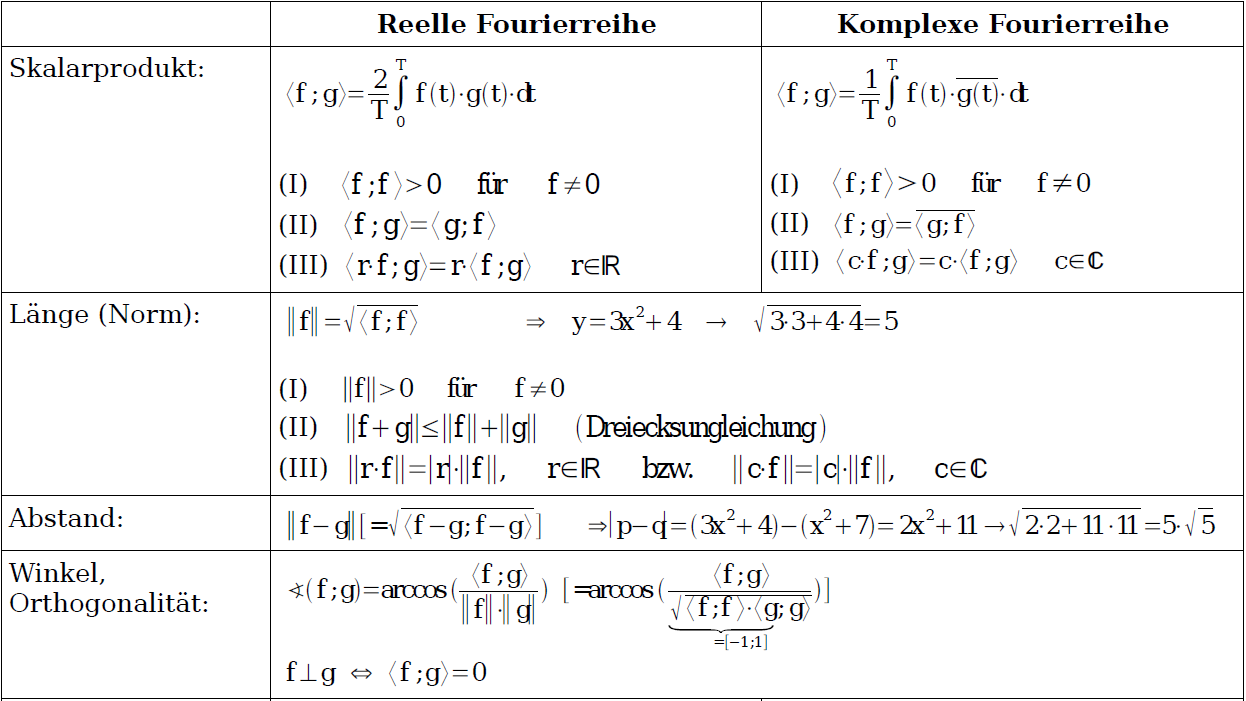
\includegraphics[width=6cm]{./bilder/vektor1.png}
\end{minipage}

\section{Diverses}
\begin{tabbing}
	xxxxxxxxxxxxxxxxxxxxxxxxxxxx \= xxxxxxxxxxxxxxxxxxxxxxxxxxxxxx \= \kill
 	$f'(z) = \lim \limits_{\Delta z \rightarrow 0} \frac{f(z + \Delta z) -
	f(z)}{\Delta z}$ \> $(a + b)^n = \sum_{k=0}^{n} \binom n k a^{n-k} \cdot b^k$ \>
	$(a \pm b)^3 =a^3 \pm  3 a^{2} b + 3 a b^2 \pm b^3 $\\ \\
	$x_{1,2} = \frac{-b \pm \sqrt{b^2 - 4ac}}{2a}$ \> $\binom n k = \frac{n!}{k!
	\cdot (n-k)!}$ \> $(a \pm b)^4 =a^4 \pm  4 a^{3} b + 6a^2b^2 \pm 4 a b^3 +
	b^4$\\ 
	\\Partielle Integration: $\int u(x) v'(x) dx = u(x)v(x) - \int u'(x) v(x) dx$
\end{tabbing}




\end{document}
